\ifx\FORMAT\undefined
\documentclass[11pt]{book}
\usepackage{amsmath,mathtools}
\usepackage[utf8]{inputenc}
\usepackage[ngerman]{babel}
\usepackage{acronym}
\usepackage{graphicx} 
\usepackage{epstopdf}
\usepackage{svg}
\usepackage{multirow}
\usepackage{amssymb}
\usepackage{trfsigns}
\usepackage{setspace}
\usepackage{yfonts}
%\usepackage{HsKatitle11}

\onehalfspacing


%Hyperlinks package, links aus inhaltsverzeichnis
\usepackage{hyperref}
\hypersetup{
    colorlinks=false, %set true if you want colored links
    linktoc=all,
    linkbordercolor = {white}
}
%Blattformatierung
\usepackage{geometry}
\geometry{a4paper, top=25mm, left=30mm, right=25mm, bottom=20mm}

%Listing
\usepackage{courier}
\usepackage{listings}
\usepackage{color}
 \lstset{
   frame=tb,
   framexleftmargin=2.5em,
   basicstyle=\small\linespread{0.9}\bfseries\ttfamily,
   emph={square}, 
   emphstyle=\color{blue}\texttt,
   emph={[2]root,base},
   emphstyle={[2]\color{yac}\texttt},
   showstringspaces=false,
   flexiblecolumns=false,
   tabsize=2,
   numbers=left,
   numberstyle=\small\bfseries\ttfamily,
   numberblanklines=false,
   stepnumber=1,
   numbersep=10pt,
   xleftmargin=25pt
 }
 
 \def\presuper#1#2%
	{\mathop{}%
	\mathopen{\vphantom{#2}}^{#1}%
	\kern-\scriptspace%
	#2}
%Display vecotr in a reference frame
\newcommand{\vecBS}[4]{\presuper{#1}{\begin{pmatrix}
#2 \\ #3 \\ #4
\end{pmatrix}}}
%Boldsymbol shortcut
\newcommand{\bs}[1]{\boldsymbol{#1}}
%Bezugssystemdefinition
\newcommand{\defBS}[1]{\{#1\} [ \bs{e}_{{#1}_1},\bs{e}_{{#1}_2}, \bs{e}_{{#1}_3} ]}
%Projektionsmatrix
\newcommand{\pMat}[2]{\presuper{#1}{\bs{P}}^{#2}}
%Differenation in Respekt zu BS
\newcommand{\diffIn}[3]{\frac{\presuper{#1}{d{#2}}}{d#3}}
\newcommand{\partialDiffIn}[3]{\frac{\presuper{#1}{\partial{#2}}}{\partial #3}}
%Geschwindigkeit/Beschleunigung
\newcommand{\vel}[3]{\presuper{#1}{\bs{#2}}^{#3}}

%Rightarrow with spaceing
\newcommand{\rArrow}{\hspace{5pt}\rightarrow\hspace{5pt}}
%Inneres Produkt
\newcommand{\inProd}[2]{\langle {#1}, {#2} \rangle}

%System macro
\newcommand{\cSS}[3]{\textfrak{S}($\bs{#1}$,$\bs{#2}$,$\bs{#3}$)}
\newcommand{\dSS}[3]{\textfrak{D}($\bs{#1}$,$\bs{#2}$,$\bs{#3}$)}

%Laplace transform sign with spaces
\newcommand{\myLaplace}{\hspace{15pt}\laplace\hspace{15pt}}

\newcommand*{\signed}[1]{%
        \nolinebreak[3]\hspace*{\fill}\mbox{\emph{#1}}
    }
\begin{document}
\fi

\chapter{Implementierung des Regelungskonzeptes}\label{chapter_SW}
Wie bereits in den letzten Abschnitten erläutert, wird der Regler als diskretes System implementiert. Deshalb spielt die verwendete Hardware und darauf ausgeführte Software eine zentrale Rolle. Dieser Umstand wird dadurch verstärkt, dass sämtliche Versuche, wie z.B. die Justierung der Sensoren, Systemidentifikation und Erprobung verschiedener Reglerkonzepte, in Form eines Programms durchgeführt werden. Aus diesem Grund widmet sich dieser Abschnitt dem Aufbau einer Software-Infrastruktur, welche die effiziente Entwicklung von mechatronischen Anwendungen ermöglicht.

\newpage
\section{Zielplattform, Sensorik und Aktorik}
In diesem Projekt wird ein BeagleBone Black\footnote{Im weiteren wird die Kurzform BeagleBone bzw. die Abkürzung BBB verwendet.} \cite{BBBSRM} in Kombination mit einer Linux-Distribution verwendet um die digitale Regelung zu realisieren. Die Plattform basiert auf einem AM335x Sitara  Prozessor \cite{AM335x}, der mit einer Taktrate von 1GHz betrieben wird. Des weiteren steht eine single precision NEON FPU, für die Berechnung von Gleitkommaoperationen, zur Verfügung. Diese Plattform reduziert die nötige Rechenzeit für gewöhnliche Filter- und Regelungsalgorithmen auf wenige Mikrosekunden. Somit kann die durch die Berechnung resultierende Totzeitbei dem Reglerentwurf vernachlässigt werden.
Das Linux-Betriebssystem bringt weitere Vorteile für die Entwicklung des Gesamtsystems mit sich. Zunächst existiert eine Vielzahl von Werkzeugen für die Entwicklung von Embbeded-Linux-Anwendungen. Dadurch wird der nötige Zeitaufwand für die Implementierung des Reglerprogramms reduziert. Des weiteren kann bei der Entwicklung auf Pakete und Bibliotheken der Linux-Gemeinde zurückgegriffen werden. Somit können auch komplexe Subsysteme, wie z.B. der hier verwendete TCP/IP-Server, in das Gesamtsystem eingebettet werden. Zuletzt kann das Dateisystem genutzt werden um Konfigurationen für Filter- und Regleralgorithmen auszutauschen, wodurch die Erprobung von verschiedenen Reglerkonzepten vereinfacht wird. 
Allerdings muss der Einfluss des Betriebssystem auf das Zeitverhalten der Regelung kritisch betrachtet werden. Einerseits kann die Abtastung an äquidistanten Stützstellen nicht mehr garantiert werden. Anderseits entsteht durch die Verwendung von Linux-Treibern Verzögerungen, die zu weiteren Totzeiten führen.

Aus diesem Grund wird zunächst die verwendete Peripherie und deren softwareseite Auswertung vorgestellt. Auf dem Würfelgehäuse sind insgesamt sechs MPU9250-Module \cite{MPU9250} montiert. Die Module besitzen jeweils einen Beschleunigungs- und Drehratensensor, welche genutzt werden um einen Teil des Zustandvektors zu bestimmen. Die Kommunikation zwischen den Sensormodulen und dem BeagleBone Black erfolgt über einen SPI-Bus. Das das SPI-Modul des BeagleBone Black nur einen CS-Pin besitzt, wird dieser über einen Analogschalter \cite{MAX4617} mit den Sensoren verbunden.
\begin{figure}[!h]
\centering
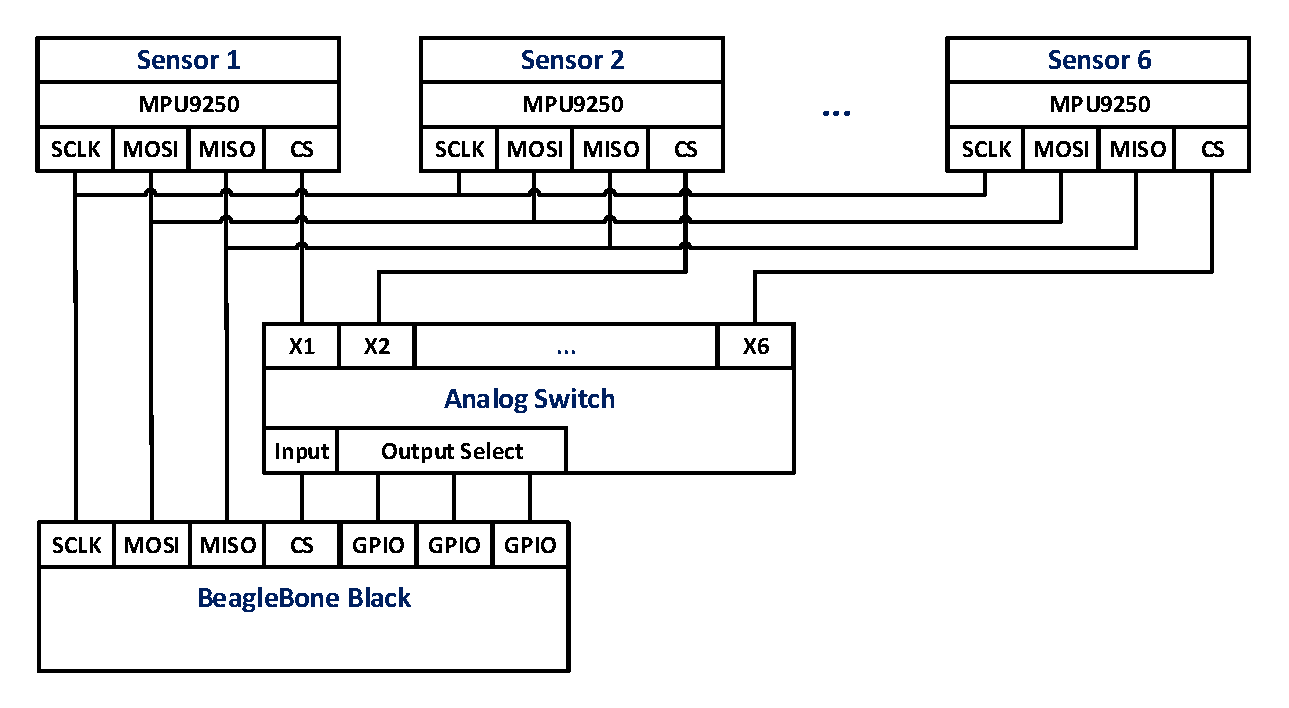
\includegraphics[width=0.7\linewidth]{img/SW_0_Sensoren_BSB.pdf}
\caption{Blockschaltbild Sensorkommunikation}
\end{figure}
Drei digitale Ausgänge des BealgeBone sind mit den Steuereingängen des Schalters verbunden um die CS-Leitung auf den Ausgang des gewünschten Sensors zu legen.
Im Quellcode werden die Peripheriegeräte durch Klassen repräsentiert. Für die Steuerung der Digitalausgänge wird die Klasse \textit{CGPIO} implementiert, welche als Konstruktorargument die Nummer des zu konfigurierenden Pins entgegennimmt. Des weiteren bietet sie Methoden zum Setzen bzw. Rücksetzen des Ausgangs. Hierfür wird die Schnittstelle des Treibers im Dateisystem verwendet. Zur Steuerung des Schalters wird die Klasse \textit{CSwitch} aus drei Instanzen des Typs \textit{CGPIO} komponiert und implementiert die Methoden \textit{selectXi()} um die Schalterausgänge auszuwählen.
Analog wird für die Konfiguration und Auswertung der Sensoren die Klasse \textit{CMPU9250} implementiert. Zur Interaktion mit dem SPI-Treiber wird die Posix-Funktion \textit{ioctl()} verwendet, welche zu einer kürzeren Ausführungszeit der Treiberaufrufe führt und im Vergleich zu der Dateisystemschnittstelle detaillierte Konfigurationsoptionen bietet. Die Klasse nutzt die SPI-Schnittstelle um die Sensoren in der \textit{init()}-Methode zu konfigurieren. Anschießend können über die Methode \textit{fetchData()} die aktuellen Beschleunigungs- und Winkelgeschwindigkeitswerte ausgelesen werden.

Die letztendliche Anwenderschnittstelle bietet die Klasse \textit{CSensorSystem}, welche aus einer Instanz des Typ \textit{CSwitch} und \textit{CMPU9250} komponiert wird. Im Konstruktur werden die sechs Sensoren initialisiert und anschließend über die Methode \textit{fetchSensorData()} ausgelesen. Die Daten werden in der Struktur \textit{SSensorData} gespeichert, welche Membervariablen für die Messwerte besitzt.
\begin{figure}[!h]
\centering
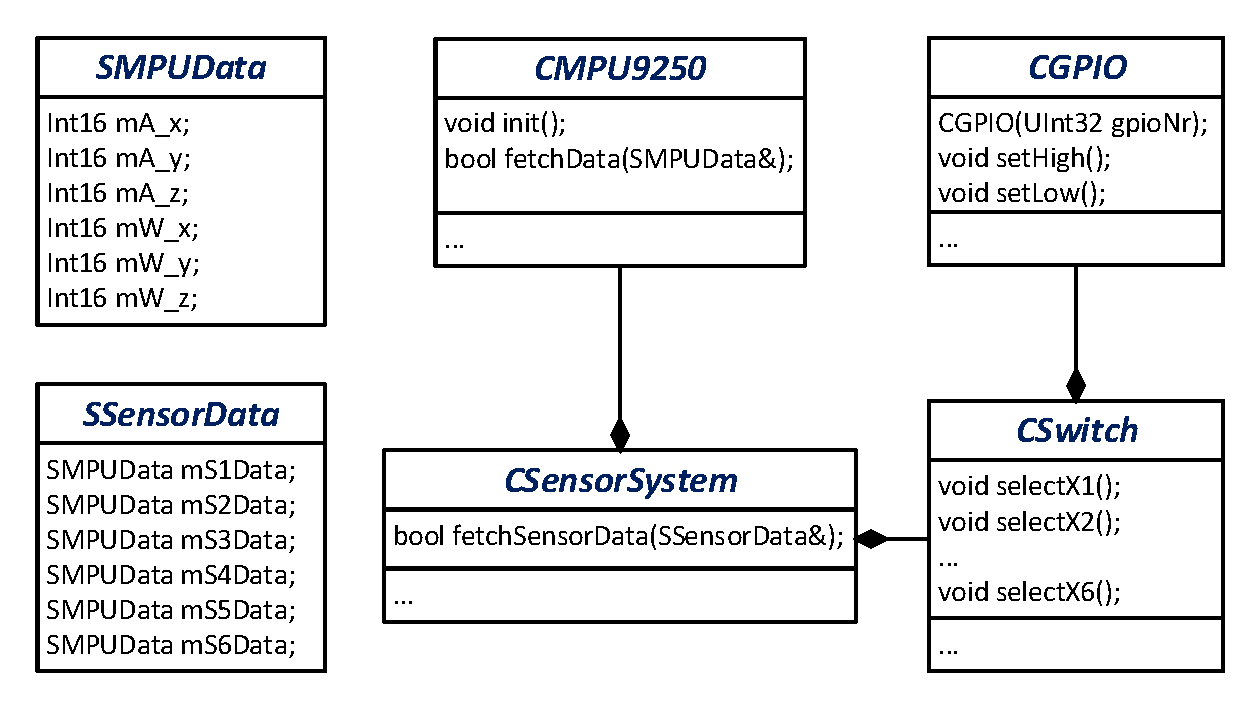
\includegraphics[width=0.7\linewidth]{img/SW_0_Sensoren_KD.pdf}
\caption{Klassendiagramm der Sensorschnittstelle}
\end{figure}

Die Stellgrößen der Regelung werden durch drei Motoren generiert, die jeweils über einen Treiberbaustein kontrolliert werden. Jeder Motortreiber ist mit zwei digitalen Ausgängen verbunden. Diese steuern die Freigabe und Drehrichtung des Motors. Die Vorgabe des Drehmoments erfolgt über ein PWM-Signal. Zusätzlich erfassen die Motortreiber die Drehzahl und geben diese in Form eines Analogsignals an das BeagleBone zurück.
\begin{figure}[!h]
\centering

\includegraphics[width=0.7\linewidth]{img/SW_0_Motoren_BSB.pdf}
\caption{Blockschaltbild der Motoransteuerung} 
\end{figure}
Die Klasse \textit{CPWM} ermöglicht das Setzen eines Duty-Cycles, wobei die Treiberschnittstelle im Dateisystem verwendet wird. Eine Instanz dieser Klasse wird in \textit{CMotor} genutzt um das gewünschte Drehmoment einzustellen. Des weiteren werden zwei Instanz von \textit{CGPIO} genutzt um die Freigabe und Drehrichtung des Motors einzustellen. Für das Auslesen der ADC-Werte wird ebenfalls eine Klasse \textit{CADC} angelegt. Da der Linux-Treiber für die Nutzung der AD-Wandler teilweise fehlerhaft ist wird ein alternative Vorgehensweise zur Nutzung der Peripherie genutzt. Hierbei wird mittels der Posix-Funktion \textit{mmap()} der Adressbereich der ADC-Peripherie in den Userspace gelegt. Dadurch kann in der Anwendung direkt auf die ADC-Register zugegriffen werden. Durch diesen Ansatz ergeben sich zwei Vorteile. Einerseits werden dem Nutzer keine Einschränkungen durch die Treiberschnittstelle aufgezwungen. Andererseits wird die nötige Zeit der AD-Wandlung durch den direkten Zugriff auf die Register reduziert. Allerdings ist diese Vorgehensweise mit einem größeren Implementierungsaufwand verbunden und wird deshalb nur genutzt wenn die Einschränkungen des Treibers nicht annehmbar sind.
die Klasse \textit{CSensorSystem} wird um eine Instanz von \textit{CADC} erweitert und umfasst somit die vollständige Sensorik des Systems. Um die Peripherie vollständig zu kapseln wird die Klasse \textit{CHardware} aus einer Instanz von \textit{CMotor} und \textit{CSensorSystem} komponiert.
\begin{figure}[!h]
\centering
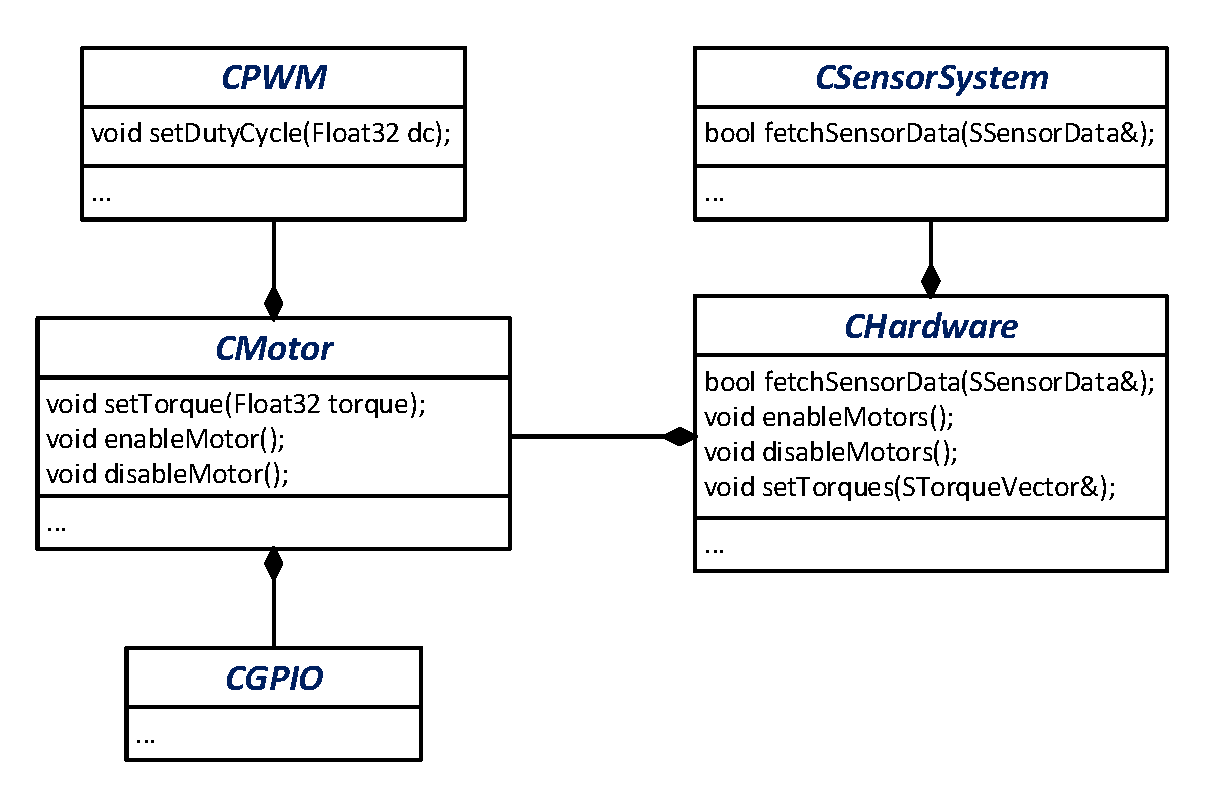
\includegraphics[width=0.7\linewidth]{img/SW_0_Hardware_KD.pdf}
\caption{Klassendiagramm der Hardwareansteuerung}
\end{figure}
\newpage
\section{Implementierung des Signalflusses}
Im nächsten Schritt muss der Signalfluss implementiert werden. Hierfür wird ein Ansatz der Template-Metaprogrammierung verwendet, um ein einheitliches Konzept für die Umsetzung von Singalverarbeitungsalgorithmen zu schaffen. Ebenso soll das Konzept Änderung im Singalfluss ermöglichen, ohne dabei größere Eingriffe im Quellcode vornehmen zu müssen. Als Beispiel wird das folgende Blockschaltbild verwendet.
Zunächst wird eine, auf den Sensorwerten basierende, Zustandsschätzung durchgeführt. Dieser Vektor wird anschließend gefiltert und zur Berechnung des Reglers genutzt.
\begin{figure}[!h]
\centering
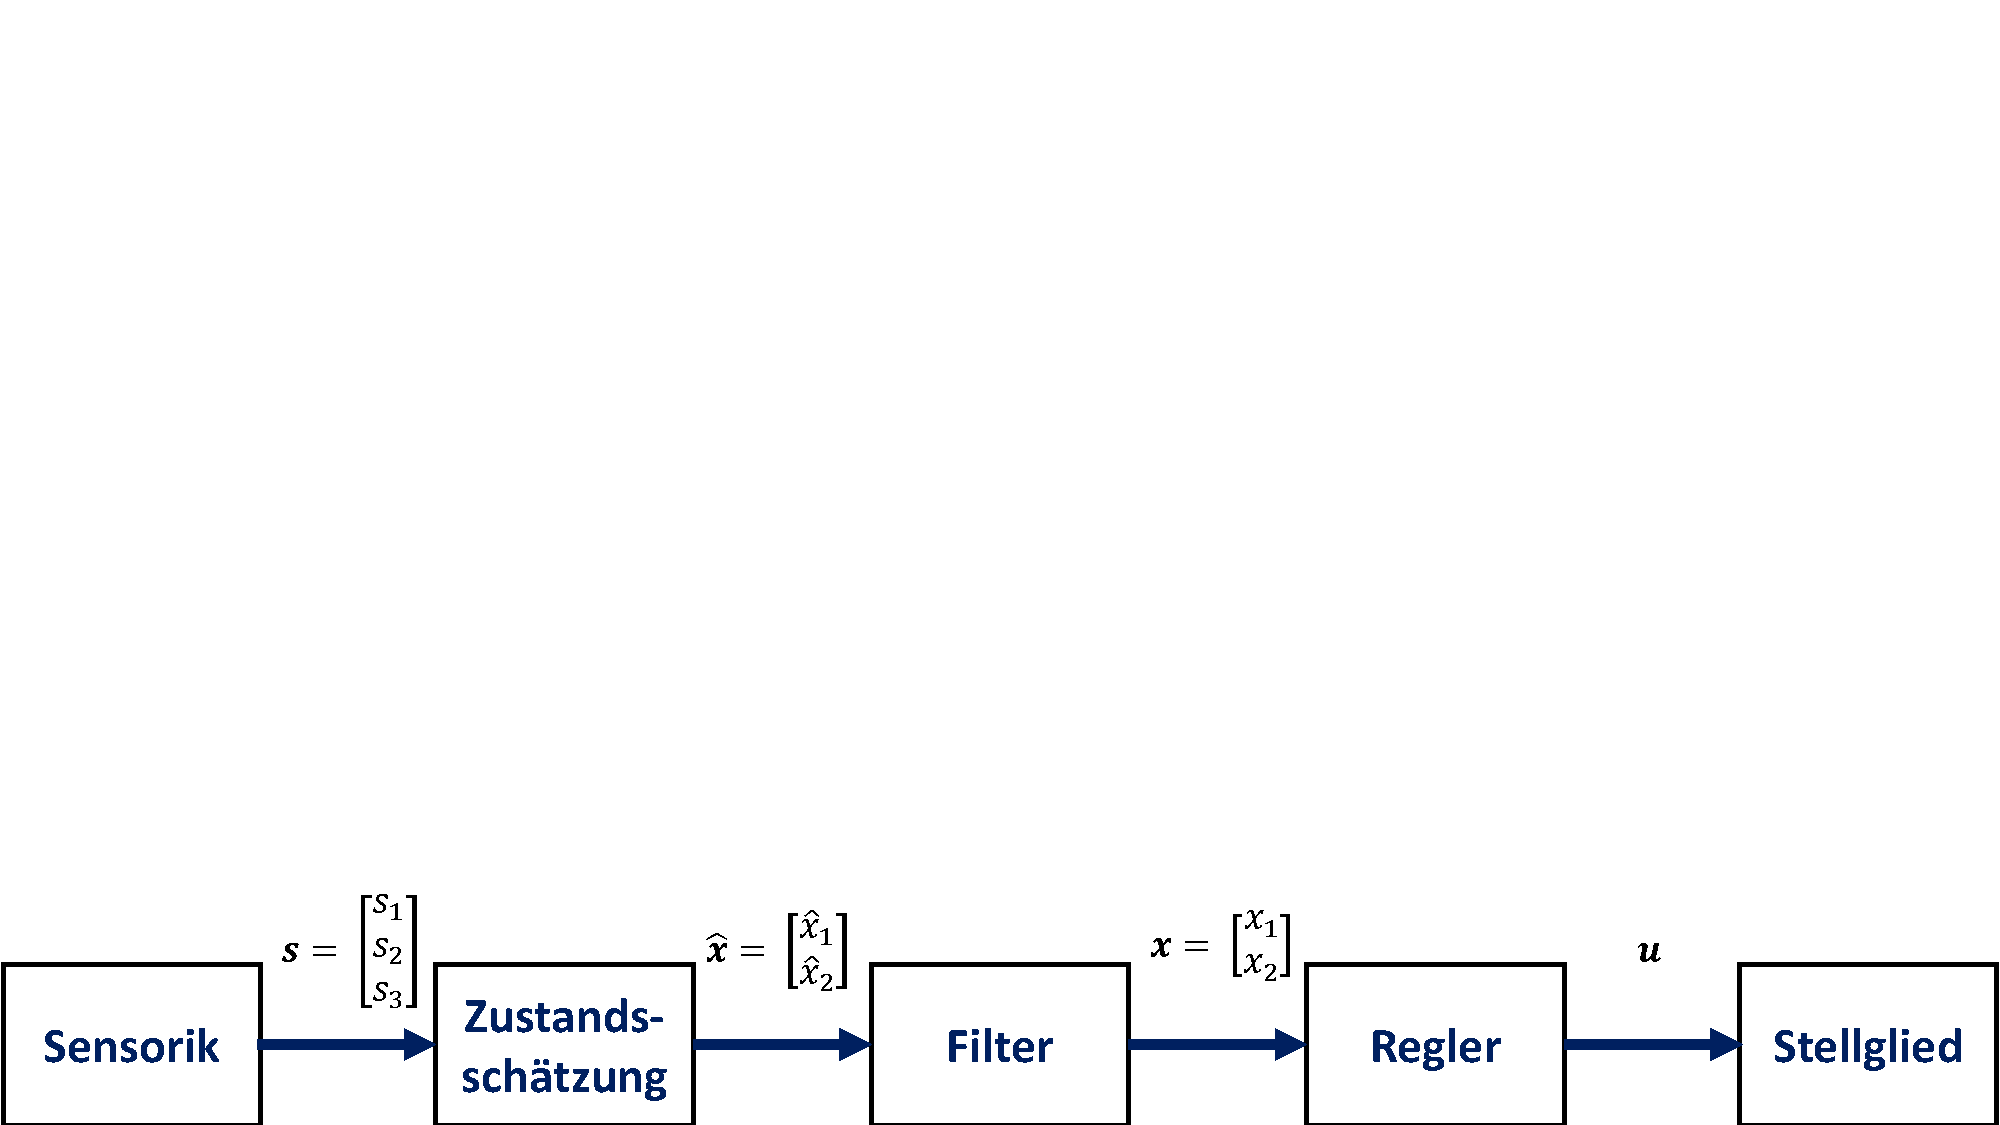
\includegraphics[width=0.9\linewidth, trim={0cm 0cm 0cm 14cm}, clip]{img/SW_1_Signalfluss_BSB.pdf}
\caption{Blockschaltbild des Signalflusses}
\end{figure}

Für die Implementierung werden die Signale als Datenobjekte implementiert. Das heißt es werden Strukturen oder Klassen entworfen, welche die Daten enthalten und ggf. Methoden für den Zugriff oder Bearbeitung bieten. Für dieses Beispiel repräsentieren die Strukturen \textit{SSensorData} und \textit{SStateVector} den Sensor- bzw. Zustandsvektor. Für die Modellierung der Stellgröße genügt eine \textit{float}-Variable.
\begin{lstlisting}[caption={Beispielhafte Implementierung eines Datenobjektes},captionpos=b]
struct SSensorData
{
	Float32 mS1;
	Float32 mS2;
	Float32 mS3;
};
struct SStateVector
{
	Float32 mX1;
	Float32 mX2;
};
using UType = Float32;
\end{lstlisting}
Die Systeme im Signalfluss werden als Klassen implementiert, die als Aktionsobjekte bezeichnet werden. Die Klassen werden nach dem folgenden Schema entworfen, wobei als Beispiel ein Objekt zur Zustandsschätzung aufgezeigt wird.
\begin{lstlisting}[caption={Beispielhafte Implementierung eines Aktionsobjektes},captionpos=b]
class CStateEstimate
{
public:
	using InputType	 = SSensorData;
	using OutputType = SStateVector;
public:
	const OutputType& calcOutput(const InputType& input);
	const OutputType& getValue() const;
	...
private:	 
	OutputType mOutput;
};
\end{lstlisting}
Die Aktionsobjekte definieren zunächst ihren Ein- und Ausgangstyp. Die Berechnung des Systems erfolgt über die Methode \textit{calcOutput()}.
Nun müssen die Aktionsobjekte zu dem vorgegebenen Signalfluss zusammengefasst werden. Um diesen Schritt im Entwicklungsprozess zu erleichtern, soll ein Konzept implementiert werden, dem eine Typenliste der Aktionsobjekte übergeben wird und daraus das Blockschaltbild erzeugt.
Für die Implementierung der Typenliste wird der Ansatz nach \cite[S. 40 ff.]{ModernCpp} verwendet. Zunächst wird die leere Struktur \textit{CNullType} definiert, welche als Terminierungssymbol in der Typenliste fungiert. Die Liste wird mit Hilfe der Templatestruktur \textit{TTypeList} implementiert, welche als Parameter einen Anfangs- und Endtypen entgegennimmt.
\begin{lstlisting}[caption={Implementierung der Typenlist},captionpos=b]
struct CNullType{};

template<class HeadType, class TailType>
struct TTypeList
{
	using Head = HeadType;
	using Tail = TailType;
};
\end{lstlisting}
Die obige Implementierung unterstützt lediglich Listen der Länge zwei. Deshalb werden Makros verwendet \cite[S. 45]{ModernCpp}, die rekursive Intanszierungen des Templates nutzen um die Listen beliebiger Länge zu erhalten. Mittels dieser Makros kann dann auch die Typenliste der Aktionsobjekte erzeugt werden.
\begin{lstlisting}[caption={Definition und Aufruf der Makors für verlängerte Typenlisten},captionpos=b]
#define TYPELIST_1(T1)         TTypeList<T1, CNullType>
#define TYPELIST_2(T1, T2) 	   TTypeList<T1, TYPELIST_1(T2)>
#define TYPELIST_3(T1, T2, T3) TTypeList<T1, TYPELIST_2(T2, T3)>
...
using ActionObjList = TYPELIST_3(CStateEstimate, CFilter, CController);
\end{lstlisting}
Um nun die Aktionstypen zu einem Signalfluss-Objekt zusammenzufügen, wird das Muster der linearen Typenhierachie nach \cite[S. 62 ff.]{ModernCpp} angewandt. Dessen Aufbau erinnert an eine verkettete Liste, wobei die Typen durch Vererbung verknüpft werden. Die Templateklasse \textit{TActionHolder} wird als Träger für die Aktionsobjekte entworfen.
Im allgemeinen Fall wird dem Template der Typ eines Aktionobjektes \textit{ActionObj} und eine beliebige Elternklasse \textit{Base} übergeben, die beide an \textit{TActionHolder} vererben. In der \textit{calcOutput()}-Methode wird zunächst die Berechnung des Aktionsobjektes durchgeführt und anschließend \textit{calcOutput()} der zweiten Elternklasse aufgerufen.
\begin{lstlisting}[caption={Templateklasse des Trägerobjektes},captionpos=b]
template<class ActionObj, class Base>
class TActionHolder : public Base, public ActionObj
{
public:
	void calcOutput(const ActionObj::InputType& input)
	{
		ActionObj::calcOutput(input);
		Base::calcOutput(ActionObj::getValue());
	}
};
\end{lstlisting}
Des weiteren besteht eine Templatespezialisierung für den Fall, dass ein Aktionstyp und \textit{CNullType}, der das Ende der Typenliste signalisiert, übergeben werden. Nun wird in der \textit{calcOutput()}-Methode lediglich das Aktionsobjekt berechnet, da das Ende der Typenliste und somit des Signalflusses erreicht ist.
\begin{lstlisting}[caption={Templatespezialisierung des Trägerobjektes für das Ende der Typenliste},captionpos=b]
template<class ActionObj>
class TActionHodler<ActionObj, CNullType> : 
	public CNullType, public ActionObj
{
public:
	void calcOutput(const ActionObj::InputType& input)
	{
		ActionObj::calcOutput(input);
	}
};
\end{lstlisting}
Die zweite Templateklasse ist \textit{TLinHierachy}, mit dem folgenden Prototyp.
\begin{lstlisting}[caption={Deklaration der Templateklasse für lineare Hierarchien {\cite[S. 63]{ModernCpp}} },captionpos=b]
template<class TList,
         template<AtomicType, class Base> class Unit,
         class Root = CNullType>
class TLinHierachy;
\end{lstlisting} 
Der erste Templateparameter ist die Typenliste, welche die zu generierende Typenhierachie vorgibt. Der zweite Parameter ist eine Templateklasse, die als Träger der Objekte aus der Typenliste agiert. In diesem Anwendungsfall wird die zuvor definierte Templateklasse \textit{TActionHolder} verwendet. Der letzte Parameter ist der Terminierungstyp der Hierarchie, welcher als Standardargument \textit{CNullType} übergeben wird. Analog zu \textit{TActionHolder} werden durch Spezialisierungen zwei Fälle unterschieden. Zunächst sei der Fall betrachtet, dass der Parameter \textit{TList} eine Typenliste aus zwei beliebigen Typen ist.
\begin{lstlisting}[caption={Erste Templatespezialisierung der linearen Hierarchie {\cite[S. 64]{ModernCpp}} },captionpos=b]
template<class T1, 
         class T2, 
         template<class, class> class Unit, 
         class Root>
class TLinHierachy<TTypeList<T1, T2>, Unit, Root>
	: public Unit<T1, TLinHierachy<T2, Unit, Root> >
{};
\end{lstlisting}
Diese Instanziierung wird solange genutzt bist das Ende der ursprünglichen Typenliste erreicht ist. Die instantiierte Klasse von \textit{TLinHierachy}, ist eine leere Klasse die von \textit{Unit} erbt. \textit{Unit} wird wiederum mit \textit{TLinHierachy} instantiiert, wobei lediglich der zweite Parameter \textit{T2} übergeben wird. Dadurch wird die ursprüngliche Typenliste schrittweise abgearbeitet.
Die zweite Templatespezialisierung wird genutzt um die Generation am Ende der Typenliste zu terminieren. Dies ist der Fall wenn \textit{TLinHierachy} mit einer Typeliste der Länge eins instantiiert wird.
\begin{lstlisting}[caption={Zweite Templatespezialisierung der linearen Hierarchie {\cite[S. 64]{ModernCpp}} },captionpos=b]
template<class T, template<class, class> class Unit, class Root>
class TLinHierachy<TYPELIST_1(T), Unit, Root>
	: public Unit<T, Root>
{};
\end{lstlisting}
Für das hier aufgeführte Beispiel ergibt sich die folgende Vererbungshierarchie.
\begin{figure}[!h]
\centering
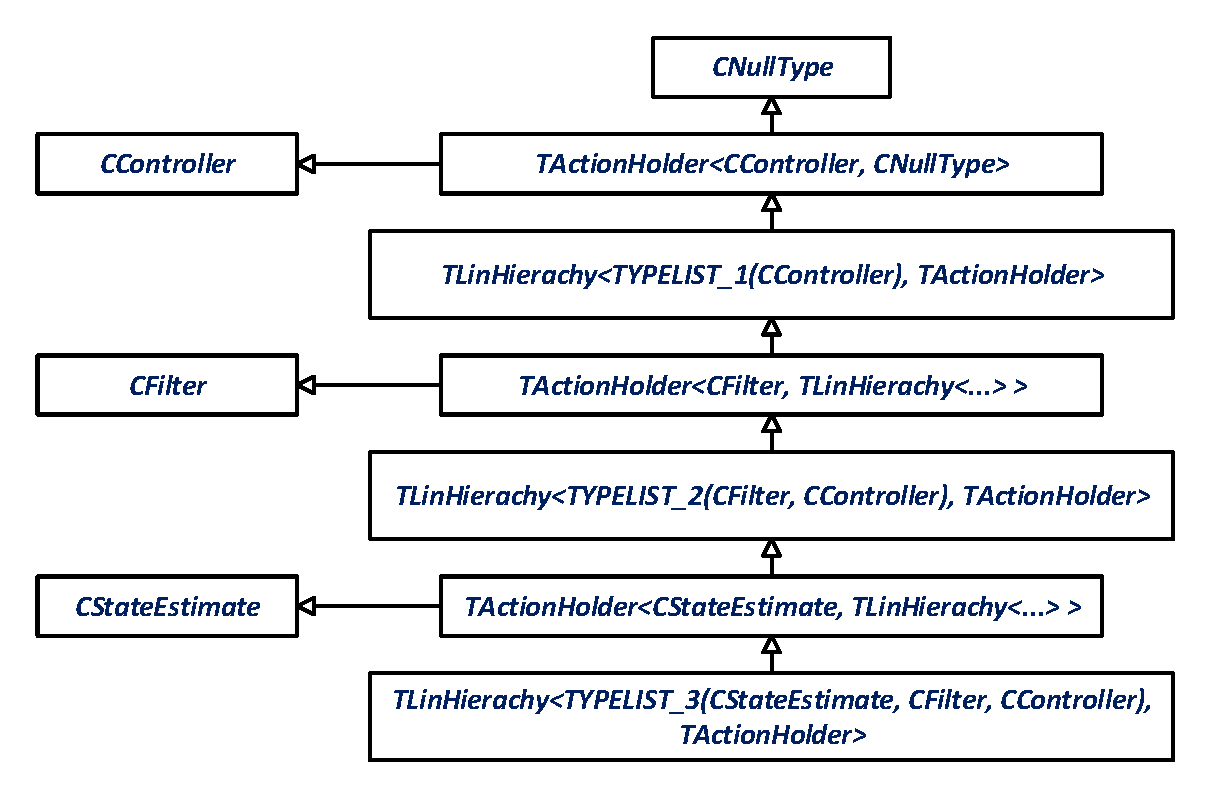
\includegraphics[width=0.7\linewidth]{img/SW_1_Signalfluss_KD.pdf}
\caption{Klassendiagramm der generierten Hierarchie}
\end{figure}
Der Vorteil dieses Konzept, welches mit einem nicht zu vernachlässigenden Programmieraufwand verbunden ist, zeigt sich bei der letztendlichen Nutzung. Sind die Aktionsobjekte definiert können sie in wenigen Zeilen zu dem Signalfluss zusammengesetzt werden.
\begin{lstlisting}[caption={Anwendungsbeispiel der linearen Hierarchie},captionpos=b]
using ActionList = TYPELIST_3(CStateEstimate, CFilter, CController);
using SignalFlow = TLinHierachy<ActionList, TActionHandler>;
SignalFlow mySF;
\end{lstlisting}
Sollen nun im Projektverlauf einzelne Elemente ausgetauscht oder erweitert werden muss lediglich die Typendefinition von \textit{ActionList} geändert werden. Da die Hierarchie mittels Vererbung realisiert wird, können durch die Angabe des Namensraum die Methoden aller Elternklassen verwendet werden. Beispielsweise zeigt der folgende Ausschnitt die Abfrage aller berechneten Signale.
\begin{lstlisting}[caption={Beispiel für den Zugriff auf Aktionsobjekte in der Hierarchie},captionpos=b]
SStateVector x_estimate = mySF.CStateEstimate::getValue();
SStateVector x_filtered = mySF.CFilter::getValue();
UType        u          = mySF.CController::getValue();
\end{lstlisting}
Ebenso können zur Laufzeit konfigurierbare Elemente oder Verzweigungen implementiert werden. Angenommen zur Filterung sollen entweder ein Komplementär-Filter (\textit{CCompFilter}) oder ein Tiefpass erster Ordnung (\textit{CPT1}) genutzt werden. Dann kann eine Klasse \textit{CFilterSystem} aus diesen beiden komponiert werden, die zusätzliche Methoden zur Filterauswahl bietet.
\begin{lstlisting}[caption={Beispiel für die komponierte Aktionsobjekte},captionpos=b]
class CFilterSystem
{
public:
	using InputType  = SStateVector;
	using OutputType = SStateVector;
public:
	const OutputType& calcOutput(const InputType& input)
	{
		mCompFilter.calcOutput(input);
		mPT1Filter.calcOutput(input);
		
		return this->getValue();
	}
	const OutputType& getValue()
	{
		switch(mActiveFilter)
		{
			case EFilter::CompFilter:
				return mCompFilter.getValue();
			case EFilter::PT1Filter:
				return mPT1Filter.getValue();
			default:
				return input;
		}
	}
	void setFilter(EFilter filter)
	{
		mActiveFilter = filter;
	}
private:
	CCompFilter mCompFilter;
	CPT1        mPT1Filter;
	EFilter     mActiveFilter;
};
\end{lstlisting}
Analog können auch komplexere Verzweigungen realisiert werden, wobei \textit{TLinHierachy} zur Generation von Teilzweigen des Blockschaltbildes verwendet werden kann.
\newpage
\section{Aufbau der Komponentenarchitektur}
In dem letzten Abschnitt wurden die elementaren Funktionen des Regelkreises, wie die Peripherieinteraktion und der Signalfluss, implementiert. Um eine effiziente Versuchsdurchführung zu ermöglichen müssen allerdings weitere Funktionalitäten bereitstehen. Einerseits müssen einzelne Elemente des Regelkreises während der Ausführung konfigurierbar sein. Beispielsweise soll zwischen unterschiedlichen Regler umgeschaltet werden und einzelne Parameter geändert werden können. Des weiteren müssen die gemessen und berechneten Werte des Signalflusses an einen Entwicklungsrechner übertragen werden. Dort werden die Daten visualisiert und für eine spätere Analyse gespeichert.
Folglich muss ein Kommunikationskonzept implementiert werden um Daten zwischen der Ziel- und Entwicklungsplattform auszutauschen. Um die Berechnung des Regelkreises und die Kommunikationsaufgaben voneinander zu trennen wird eine Komponentenarchitektur eingeführt (\cite{Wietzke1}, S. 279 ff.). Die erste Komponente, welche als Regelungskomponente bezeichnet wird, führt die Berechnung des Signalflusses und die Interaktion mit den Peripheriegeräten durch. Des weiteren übernimmt sie die logische Steuerung der Versuchsabläufe. Die Kommunikationskomponente ist für die Verbindung mit dem Entwicklungsrechner verantwortlich und ermöglicht den Datenaustausch zwischen den beiden Plattform. Hierfür wird ein TCP/IP-Server verwendet.
\begin{figure}[!h]
\centering
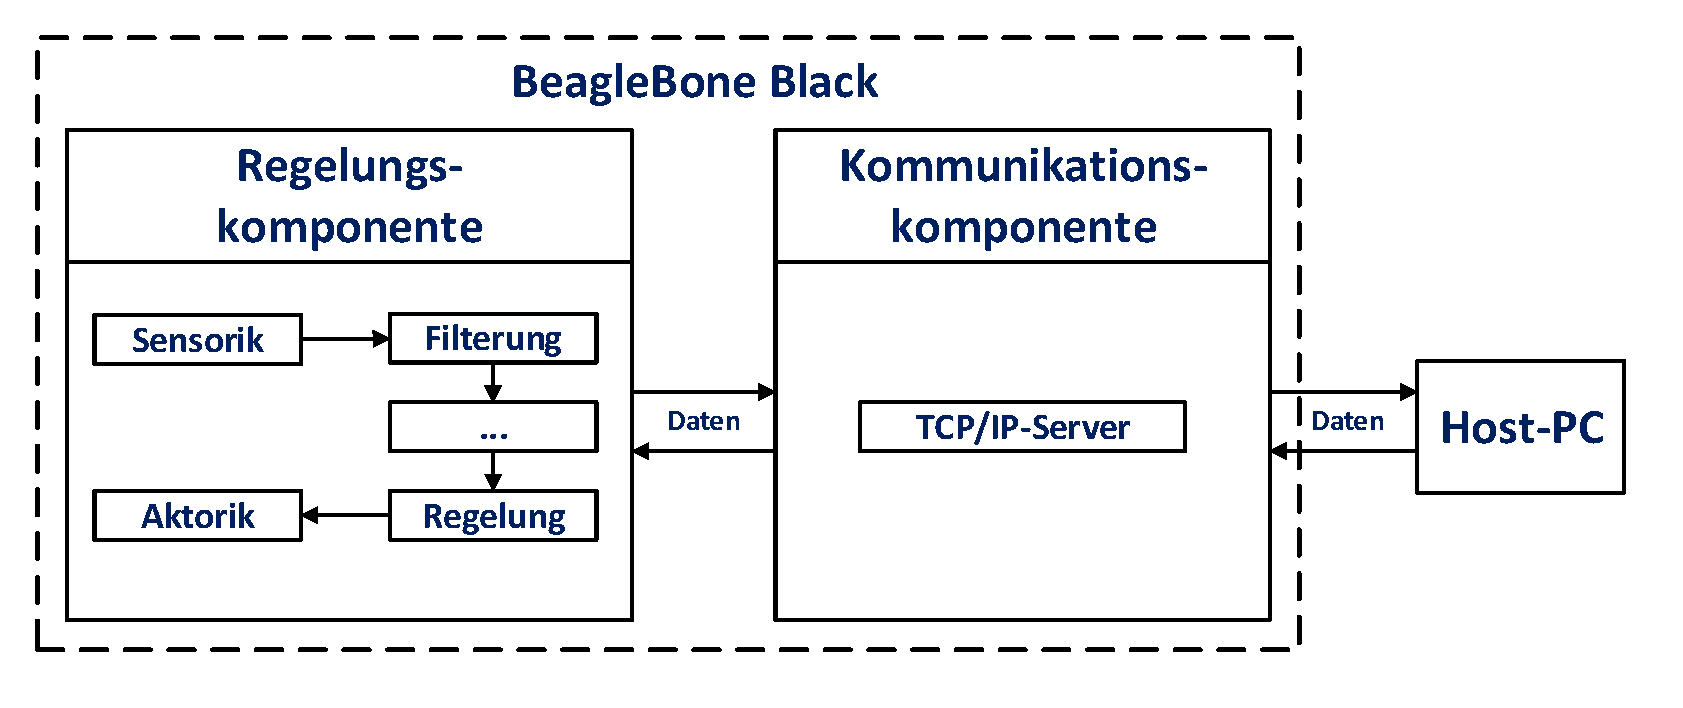
\includegraphics[width=\linewidth]{img/SW_1_KA_BSB.pdf}
\caption{Blockschaltbild Gesamtsystem}
\end{figure}
Durch die Verwendung der Komponentenarchitektur entstehen einige Vorteile. Zunächst können die beiden Komponenten in unterschiedlichen Threads ausgeführt werden. Dadurch wird die Bearbeitung der beiden Aufgabenbereiche zum Großteil entkoppelt. Der Datenaustausch zwischen den Komponenten reduziert sich auf eine kontrollierte Schnittstelle, wodurch die Fehleranfälligkeit des Gesamtsystems minimiert wird. Des weiteren können die Aufgaben priorisiert werden, da der Scheduler eine preemptive Round-Robin-Strategie verfolgt (\cite{Wietzke1}, S. 19). Somit kann die Ausführung der Regelungskomponente, welche für die Bearbeitung der zeit- und sicherheitsrelevanten Aufgaben zuständig ist, gegenüber der Kommunikationseinheit priorisiert werden. Hieraus resultiert, dass das Zeitverhalten der Regelung als deterministisch angenommen werden kann. 

Für die Implementierung wird das Interface \textit{IRunnable} definiert, welches virtuelle Methoden zur Initialisierung und Ausführung der Komponenten vorschreibt. Diese Schnittstelle wird von der abstrakten Klasse \textit{AComponentBase} geerbt, welche Membervariablen zum Datenaustausch besitzt. Die letzendlichen Komponenten werden in Form der beiden Klassen \textit{CControlComp} und \textit{CCommComp} realisiert. Die Erzeugung der Threads erfolgt mit Hilfe der Klasse \textit{CThread}, deren Instanz als Trägerobjekte der Threads agieren (\cite{Wietzke1}, S. 108 ff.).
\begin{figure}[!h]
\centering
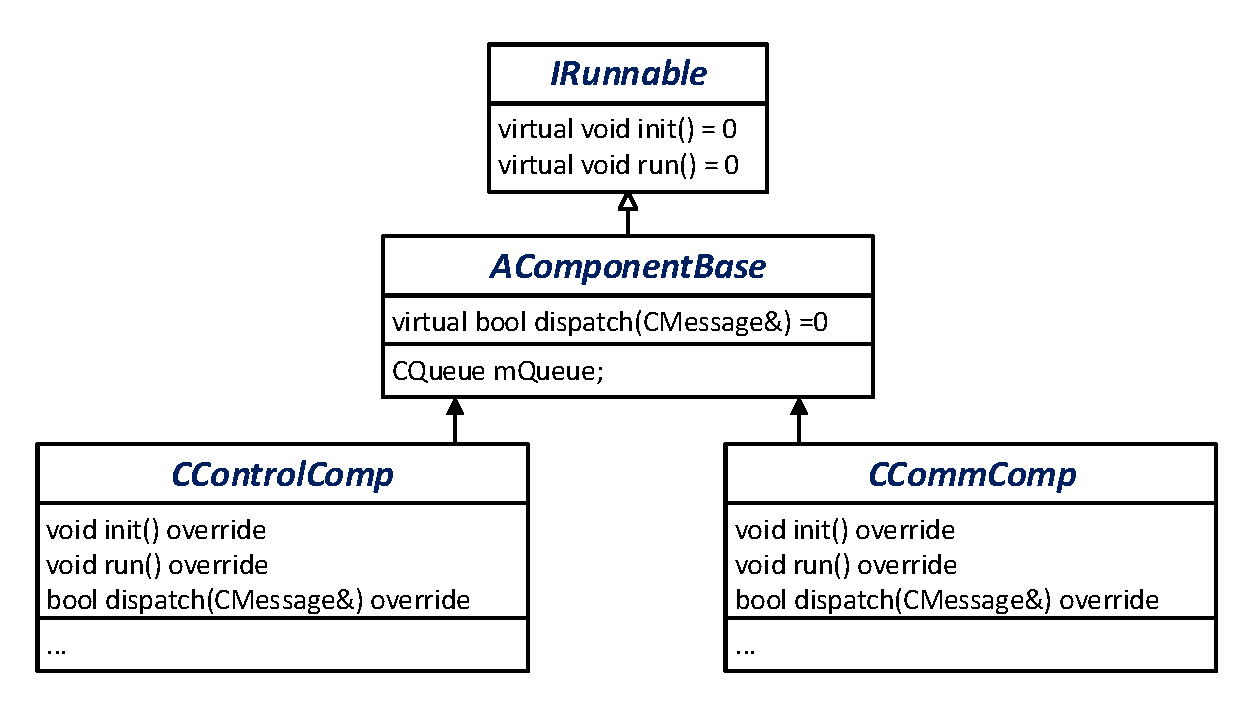
\includegraphics[width=0.6\linewidth]{img/SW_1_KA_KD.pdf}
\caption{Klassendiagramm der Komponenten}
\end{figure}

Im nächsten Schritt muss ein Weg zum Datenaustausch zwischen den Komponenten etabliert werden. Einerseits müssen Messdaten und Signale aus dem Regelkreis von der Regelungs- and die Kommunikationseinheit gesendet werden, welche diese anschließend an den Host-PC weiterleitet. Andererseits werden die Steuerbefehle des Host-PCs von der Kommunikationskomponente empfangen und an die Regelungskomponente gereicht. Da in diesem Anwendungsfall lediglich kleine Datenmengen versendet werden, werden Nachrichten für deren Austausch verwendet (\cite{Wietzke1}, S. 196). Die Nachrichten werden in Form der Klasse \textit{CMessage} implementiert, welche aus einem Datenfeld, einem Ereignis und einem Zeitstempel komponiert werden. Das Ereignis wird als Enumeration realisiert und gibt den Inhalt der Daten bzw. den jeweiligen Befehl wieder. Der Zeitstempel gibt den Abtastzeitpunkt der Signale aus dem Regelkreis wieder. 
\begin{lstlisting}[caption={Beispielhafte Implementierung der Events und Nachrichten},captionpos=b]
enum class EEvent
{
	DEFAULT_IGNORE = 0,
	TIMER_TICK     = 1,
	STATE_DATA     = 2,
	...
}
class CMessage
{
public:
	EEvent getEvent() const;
	UInt8* getDataPtr();
	...
public:

private:
	static constexpr UInt32 sDataSize = 32U;

	EEvent  mEvent;
	Float32 mTime;	
	UInt8   mData[sDataSize];
};
\end{lstlisting}
Des weiteren besitzt die Klasse \textit{CMessage}Methoden und Konstruktoren um die Datenfelder entsprechend zu füllen und auszulesen. Um die Nachrichten zu empfangen besitzen die Komponenten Eingangspuffer die als Queues implementiert werden. Die Erzeugung der Nachrichten wird von einem Proxy übernommen (\cite{Wietzke1}, S. 285 ff.), der Methoden für die unterschiedlichen Ereignisse bereitstellt. Des weiteren kennt der Proxy die Queues der Komponenten und legt neue Nachrichten, in Abhängigkeit von dem jeweiligen Event, in die Eingangspuffers des zugehörigen Empfängers.
\begin{lstlisting}[caption={Aufbau der Proxy-Klasse},captionpos=b]
class CProxy
{
	public:
		bool transmitStateVector(const StateVector& x);
		bool onTimerTick();
		bool onClientConnect();
		...
};
\end{lstlisting}
Mit Hilfe der Nachrichtenkommunikation kann auch das Ablaufschema der Komponenten verallgemeinert werden. Beim Starten der Threads werden die Komponenten zunächst über den Aufruf ihrer \textit{init()}-Methoden initialisiert, anschließend wird die \textit{run()}-Methode ausgeführt, welche in diesem Fall eine Endlosschleife darstellt. In einem Durchlauf wird geprüft ob neue Nachrichten vorhanden sind, trifft dies zu wird die Nachricht über die \textit{dispatch()}-Methode verarbeitet. Andernfalls legt sich der Thread schlafen bis neue Nachrichten zur Verfügung stehen. Hieraus ergeben sich zwei Vorteile. Einerseits werden die Komponenten nach einem einheitlichen Konzept entworfen, lediglich die Implementierung der \textit{init()}- und \textit{dispatch()}-Methode unterscheiden sich, andererseits wird durch die Synchronisation der Komponenten deren Laufzeit reduziert.
\newpage
\section{Entwurf der Regelungskomponente}
Die Aufgabe der Regelungskomponente besteht darin den Kontroll- und Signalfluss der verschiedenen Versuche zu steuern. Diese Umsetzung erfolgt mit Hilfe eines Zustandautomats, welcher die Trennung der Kontrolllogik und der auszuführenden Aktionen ermöglicht. Des weiteren kann die Applikation bei diesem Ansatz problemlos durch weitere Versuche und Anwendungsfälle erweitert werden. 
Prinzipiell lässt sich der logische Ablauf der Komponente mit einem einfachen Zustandsdiagramm modellieren. Auf der obersten Ebene existiert ein \textit{Standby}-Zustand, der die Inaktivität der Komponente widerspiegelt. Des weiteren enthält diese Ebene Zustände für die verschiedenen Versuche. Diese werden betreten, wenn die Komponente ein Event mit dem entsprechenden Befehl zur Ausführung des Versuchs erhält.
\begin{figure}[h!]
\centering
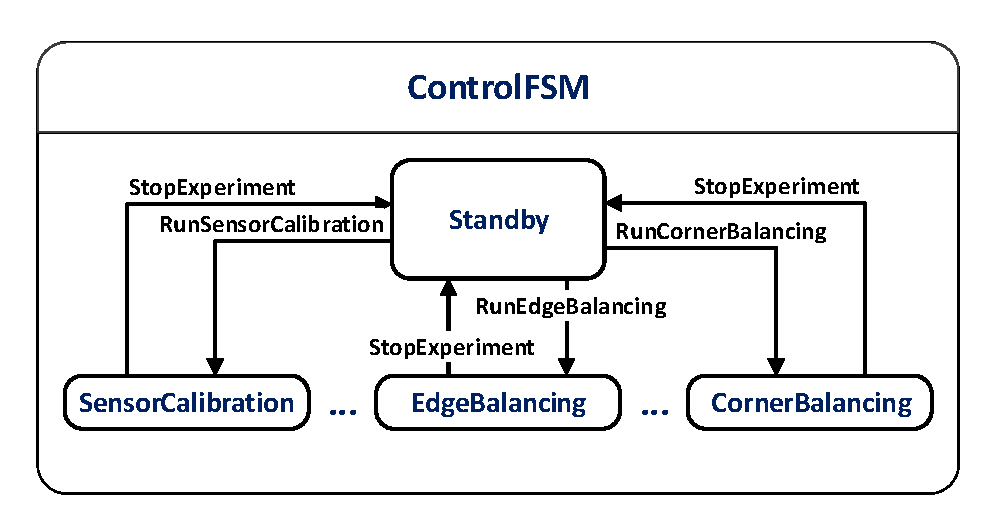
\includegraphics[width=0.7\linewidth]{img/SW_2_ControlComp_SC.pdf}
\caption{Zustandsdiagramm der Kontrol-Komponente}
\end{figure}

Ein solches Zustandsdiagramm kann z.B. mit einer objektorientierten Adaption der Methode von Samek \cite[S. 246 ff.]{Wietzke1} implementiert werden. Hierbei werden Zustände als Methoden der FSM realisiert, wobei für Oberzustände eigene Klassen entworfen werden, die wiederum Methoden für die jeweiligen Unterzustände besitzen. Die Referenzierung des aktuellen Zustandes erfolgt über einen Funktionenzeiger, der auf die Methode des entsprechenden Zustandes gerichtet ist. 

Als Basis der Typenhierachie dient die abstrakte Klasse \textit{AState}, welche den Zustandstypen als Methodenzeiger definiert, eine Standardimplementierung der \textit{dispatch()}-Methode vorgibt und statische Membervariablen deklariert um die Verarbeitung interner Events zu ermöglichen.
\begin{lstlisting}[caption={Abstrakte Basisklasse für die Zustände},captionpos=b]
class AState
{
protected:
	using StatePtr = bool (AState::*)(CMessage&);
public:
	virtual bool onInitial(CMessage& msg) = 0;
	virtual bool dispatch(CMessage& msg);
	...
protected:
	StatePtr mStatePtr;
	static constexpr StatePtr sInitial = 
			static_cast<StatePtr>(AState::onInitial);
	static CMessage sInternalQueue;
	static UInt32   sQueueSize;
};
\end{lstlisting}
Die Methode \textit{onInitial()} wird verwendet um die FSM und Oberzustände über ein \textit{Init}-Event zu initialisieren. Die \textit{dispatch()}-Methode beschränkt sich auf den Aufruf des aktuellen Zustands.

\begin{lstlisting}[caption={Defintion der \textit{dispatch()}-Methode},captionpos=b]
bool AState::dispatch(CMessage& msg)
{
	return *(this->mStatePtr)(msg);
}
\end{lstlisting} 

Die auszuführenden Aktionen, wie z.B. die Berechnung des Regelkreises, werden in der Klasse \textit{CActionHandler} gekapselt \cite[S. 225]{Wietzke1}. Dadurch erfolgt eine klare Trennung des Kontroll- und Signalflusses. Prinzipiell besitzt \textit{CActionHandler} Methoden, die jeweils beim Betreten und Verlassen der Zustände aufgerufen wird. Zusätzlich kann er um nötige Hilfsmethoden erweitert werden.
\begin{lstlisting}[caption={Beispielhafte Implementierung des Actionhandlers},captionpos=b]
class CActionHandler
{
public:
	void enterStandby();
	void exitStandby();
	void enterSensorCalibration();
	void exitSensorCalibration();
	...
	void sampleSensorCalibration();
	void sampleEdgeBalancing();
	...
private:
	CThread    mTimerThread;
	CTimerTask mTimerTask;
	
	CHardware         mHardware;
	EdgeBalancingSF   mEdgeBalancingSF;
	ConrnerBalacingSF mCornerBalacingSF;
};
\end{lstlisting}
Für die Zeitgebung wird einer separater Timer-Task \textit{CTimerTask} verwendet, der von \textit{CActionHandler} verwaltet wird. Die Timerklasse kann mittels der Methoden \textit{pause()} und \textit{resume()} pausiert bzw. gestartet werden. Während der Ausführung schläft der Timer für eine konfigurierbare Abtastzeit und erzeugt anschließend über den Proxy ein \textit{TimerTick}-Event, welches an die Regelungskomponente weitergeleitet wird.
\begin{lstlisting}[caption={Aufbau des Timer-Tasks},captionpos=b]
class CTimerTask : public IRunnable
{
public:
	void run() override
	{
		while(true)
		{
			mRunningSem.take(true);
			mRunningSem.give();
			usleep(mPeriod);
			mProxyPtr->timerTick();
		}
	}
	bool pause(bool waitForever){return mRunningSem.take(waitForever);}
	bool resume(){mRunningSem.give();}
	void setPeriod(Int32 period){mPeriod = period;};
	...
private:
	CBinarySemaphore mRunningSem;
	Int32            mPeriod;
	CProxy*          mProxyPtr;
};
\end{lstlisting}
Der Ansatz nach Samek bringt bei diesen Anwendungsfall einen Nachteil mit sich. Für die meisten Versuche genügt eine simple Kontrolllogik, weshalb diese als einfacher Unterzustand realisiert werden. Das hat eine flache Zustandshierarchie zur Folge, die der Anzahl von Versuchen entsprechend breit ist. In der Implementierung resultiert hieraus eine umfangreiche Klasse \textit{CFSM}, da diese für jeden Unterzustand um eine Methode erweitert wird. Ebenso nimmt der Umfang der Klasse \textit{CActionHandler} mit der Anzahl der Versuche kontinuierlich zu. Dieses Problem kann zwar durch die Aufteilung in mehrere Actionhandler vermieden werden, allerdings wird dadurch die Komplexität von \textit{CFSM} weiter erhöht. Diese Problematik wird dadurch verschärft, dass es sich bei der Zustandsmaschine um den Kern der Anwendung und somit kritischen Abschnitt der Anwendung handelt. Die zu Grunde liegende Komponentenarchitektur wird zu Projektbeginn erstellt und danach kaum manipuliert. Im Gegensatz dazu wird die Zustandmaschine während des Projektsverlaufes ständig verändert und erweitert, weshalb eine unübersichtliche Implementierung besonders negativ auffällt. Aus diesem Grund wird im nächsten Schritt eine alternative Vorgehensweise vorgestellt, die sich die spezielle Struktur des Zustandsdiagrammes zu Nutze macht um eine effiziente Implementierung zu schaffen.

Zunächst sei angemerkt, dass es nicht möglich ist direkt zwischen zwei Versuchszuständen zu wechseln. Ein Versuchszustand kann nur aus dem Zustand \textit{Standby} betreten werden. Des weiteren wird nach dem Verlassen eines Versuchszustandes immer in \textit{Standby} gewechselt. Dadurch kann die Kontrolllogik der Zustandsmaschine verallgemeinert werden. Ist der momentane Unterzustand nicht \textit{Standby} und es trifft ein \textit{StopExperiment}-Event ein, so wird der Zustand verlassen und in \textit{Standby} gewechselt. Befindet sich die FSM in \textit{Standby} wird bei Eintreffen eines Events geprüft ob ein Zustandswechsel erfolgen muss. Diese Prüfung kann an die Zustände abgegeben werden. Somit stellt die Zustandsmaschine in diesem Fall lediglich eine Anfrage an alle Versuchszustände ob diese betreten werden möchten.

Die Implementierung der Zustandsmaschine setzt sich folglich aus einem \textit{Standby}-Zustand und einer Liste von Versuchszuständen zusammen. Um eine übersichtliche Codestruktur zu erhalten werden diese als Klassen entworfen, die von der abstrakten Basisklasse \textit{AState} erben.
\begin{lstlisting}[caption={Angepasste Implementierung der abstrakten Zustandsklasse},captionpos=b]
class AState
{
public:
	virtual bool dispatch(CMessage&) = 0;
	virtual bool tryEntry(CMessage&, AState*&) = 0;
	virtual void onEntry() = 0;
	virtual void onExit()  = 0;
private:
	static CMessage sInternalQueue;
	static UInt32   sQueueSize;
};
\end{lstlisting}
Die Methode \textit{dispatch()} dient zur Verteilung von eintreffenden Nachrichten. Mit Hilfe von \textit{tryEntry()} kann die Zustandmaschine prüfen ob der Zustand, in Abhängigkeit des Events, betreten werden möchte. Der folgende Ausschnitt zeigt eine mögliche Implementierung für den Zustand \textit{SensorCalibration}.
\begin{lstlisting}[caption={Beispielhafte Definition der Methode \textit{tryEntry()}},captionpos=b]
bool CSensorCalibration::tryEntry(CMessage& msg, AState*& statePtr)
{
	EEvent event = msg.getEvent();
	if(EEvent::RUN_SENSORCALIBRATION == event)
	{
		statePtr = this;
		return true;
	}
	return false;
}
\end{lstlisting}
Das zweite Argument ist eine Zeigerreferenz auf den Zustandszeiger der FSM. Falls ein Zustand betreten werden soll überschreibt er die Referenz mit seinem this-Zeiger und gibt \textit{true} zurück um den Konsum des Events zu signalisieren. Die Methoden \textit{onEntry()} und \textit{onExit()} werden zum Betreten bzw. Verlassen des Zustandes verwendet. Um auch die auszuführenden Aktionen zu trennen, wird für jede Zustandsklasse ein Actionhandler implementiert. Diese erben von der Klasse \textit{CActionBase}, die gemeinsame Ressourcen als statische Membervariablen deklariert. Ein Beispiel wären hierfür Instanzen der Klassen \textit{CHardware} oder \textit{CTimerTask}.

Um die Zustandsklassen zu einer Liste zusammenzufassen wird wieder eine lineare Typenhierarchie verwendet. Hierfür muss zunächst ein Trägerobjekt \textit{TStateHolder} entworfen werden. 
\begin{lstlisting}[caption={Implementierung der Trägerklasse für Zustände},captionpos=b]
template<class State, class Base>
class TStateHolder : public Base
{
	bool tryEntry(CMessage& msg, AState*& statePtr)
	{
		bool consumed = mState.tryEntry(msg, statePtr);
		if(consumed == false)
		{
			return Base::tryEntry(msg, statePtr);
		}
		return consumed;
	}
private:
	State mState;
};
template<class State>
class TStateHolder<State, CNullType> : public CNullType
{
public:
	bool tryEntry(CMessage& msg, AState*& statePtr)
	{
		return mState.tryEntry(msg, statePtr);
	}
private:
	State mState;
};
\end{lstlisting}
Analog zu \textit{TActionHolder} wird mittels einer Templatespezialisierung unterschieden ob das Ende der Typenliste erreicht ist. Ist dies nicht der Fall wird zunächst geprüft ob der getragene Zustand betreten werden soll. Trifft dies nicht zu wird  die \textit{tryEntry()}-Methode des nächsten Elements in der Hierarchie aufgerufen. Ein Unterschied zu \textit{TActionHolder} ist, dass eine Komposition aus dem Zustandsobjekt verwendet wird. Dadurch werden die Methoden des Zustandes geschützt. Die FSM kann lediglich auf den, über ihren Zustandszeiger referenzierten, Zustand zugreifen.
Die Implementierung der Zustandsmaschine basiert ebenfalls auf einem Template, welchem die Typenliste der Versuchszustände übergeben wird. Des weiteren erbt die Templateklasse von \textit{AState} um Zugriff auf die interne Queue zu erhalten.
\begin{lstlisting}[caption={Implementierung der Templateklasse für die Zustandsmaschine},captionpos=b]
template<class StateList>
class TFSM : public AState
{
public:
	bool dispatch(CMessage& msg) override;
	bool tryEntry(CMessage& msg, AState*& statePtr) override;
	void onEntry() override;
	void onExit() override;
	bool onStandby(CMessage& msg);
	void handleUnconsumedEvent(CMessage& msg);
private:
	AState*                mStatePtr;
	TLinHierach<StateList> mStateList;
	CAction                mAction;
};
\end{lstlisting}
Neben dem Interface von \textit{AState} besitzt die Klasse zwei weitere Methoden. Wobei die erste den Zustand \textit{Standby} repräsentiert. Die zweite Methode wird genutzt um nicht konsumierte Events, was für gewöhnlich einem Fehlverhalten der FSM entspricht, abfängt. Zunächst wird die \textit{dispatch()}-Methode betrachtet. Zu Beginn wird der aktuelle Unterzustand aufgerufen. Falls das Ereignis nicht konsumiert wird und es sich um \textit{StopExperiment} handelt, wird der aktuelle Unterzustand verlassen und in \textit{Standby gewechselt}. Zuletzt wird die interne Queue abgearbeitet.
\begin{lstlisting}[caption={Definition der Methode \textit{dispatch()}},captionpos=b]
template<class StateList>
bool TFSM<StateList>::dispatch(CMessage& msg)
{
	bool consumed = false;
	if(mStatePtr == nullptr)
	{
		consumed = this->onStandby(msg);
	}
	else
	{
		consumed = mStatePtr->dispatch(msg);
	}
	
	if(consumed == false)
	{
		EEvent event = msg.getEvent();
		if(EEvent::StopExperiment == event)
		{
			mStatePtr->onExit();
			mStatePtr = nullptr;
			mAction.entryStandby();
		}
	}
	
	while(squeueSize > 0U)
	{
		CMessage internalMsg(sInternalQueue);
		sQueueSize = 0U;
		consumed = mStatePtr->dispatch(internalMsg);
	}
	return consumed;
}
\end{lstlisting}
Im Zustand \textit{Standby} wird das Ereignis an alle Unterzustände übergeben um zu prüfen, ob diese betreten werden sollen. 
\begin{lstlisting}[caption={Implementierung der Methode \textit{onStandby()}},captionpos=b]
template<class StateList>
bool TFSM<StateList>::onStandby(CMessage& msg)
{
	bool consumed = this->tryEntry(msg);
	if(consumed == true)
	{
		mAction.exitStandby();
		mStatePtr->onEntry();
	}
	return consumed;
}
\end{lstlisting}
Die Methode \textit{tryEntry()} stößt lediglich die Abfrage der Unterzustände an.
\begin{lstlisting}[caption={Implementierung der Methode \textit{tryEntry()}},captionpos=b]
template<class StateList>
bool TFSM<StateList>::tryEntry(CMessage& msg, AState*& statePtr)
{
	return mStateList.tryEntry(mg, statePtr);
}
\end{lstlisting}
Die Vorteile dieses Konzept verdeutlichen sich wieder bei der Anwendung. Für jeden Versuch wird eine Zustandsklasse und Actionhandler entworfen, wodurch eine übersichtliche Projektstruktur entsteht. Um die letztendliche Zustandsmachine zu erhalten wird lediglich \textit{TFSM} mit der gewünschten Liste von Zustandstypen instantiiert.
\begin{lstlisting}[caption={Beispielhafte Instantiierung der Zustandsmaschine},captionpos=b]
using StateList  = TYPELIST_4(CSensorCalib, CADCCalib, 
                              CEdgeBalance, CCornerBalance);
using ControlFSM = TFSM<StateList>;
ControlFSM myFSM;
\end{lstlisting}
Sollen weitere Zustände hinzugefügt oder entfernt werden muss lediglich die Typdefinition von \textit{StateList} angepasst werden. Um Coderedundanzen zu vermeiden kann für die Unterzustände auch eine Templateklasse entworfen werden, die das Eintrittsereignis und den Actionhandler als Parameter entgegennimmt. 
\begin{lstlisting}[caption={Templateklasse für einfache Versuchszustände},captionpos=b]
/* TSubState.h */
template<const EEvent entryEvent, class Action>
class TSubState : public AState
{
public:
	bool tryEntry(CMessage& msg, AState*& statePtr) override
	{
		if(entryEvent == msg.getEvent())
		{
			statePtr = this;
			return true;
		}
		return false;
	};
	bool dispatch(CMessage& msg) override;
	void onEntry() override;
	void onExit() override;
private:
	Action mAction;
};
\end{lstlisting}
Die Unterzustände spezialisieren dann lediglich die Methoden \textit{dispatch()}, \textit{onEntry()} und \textit{onExit()}, wie das folgende Beispiel zeigt.
\begin{lstlisting}[caption={Beispielhafte Instantiierung des Versuchstemplate},captionpos=b]
/* CADCCalib.cpp */
using CADCCalib = TSubState<EEvent::RunADCCalib, CADCCalibAction>;
template<>
bool CADCCalib::dispatch(CMessage& msg)
{
	EEvent event = msg.getEvent();
	if(EEvent::TIMERTICK == event)
	{
		mAction.sampleADCCalib();
		return true;
	}
	...
	return false;
}
template<>
void CADCCalib::onEntry()
{
	cout << "Entering ADC-Calibration . . . " << endl;
	mAction.resumeTimer();
}
template<>
void CADCCalib::onExit()
{
	cout << "Exiting ADC-Calibration . . . " << endl;
	mAction.pauseTimer();
}
\end{lstlisting}
\newpage
\section{Entwurf der Kommunikationskomponente}
Die zweite Komponente des Systems ist für die Kommunikation mit einem Desktop-PC verantwortlich. Unter die Kommunikationsaufgaben fällt einerseits die Übermittlung relevanter Daten des Regelkreises, wie z.B. der aktuelle Wert des Zustandvektors. Andererseits nimmt die Kommunikationskomponente Steuerbefehle entgegen und leitet diese an die Regelungskomponente weiter. Dadurch können während der Ausführung der Anwendung Konfiguration der Versuche durchgeführt werden. Beispiele hierfür sind die Auswahl des zu verwendeten Regler- oder Filterkonzeptes. Für die Verbindung zwischen der Ziel- und Entwicklungsplattform wird das TCP/IP-Protokoll verwendet, wobei die BeagleBone Black-Anwendung als Server fungiert.

Der Kontrollfluss der Kommunikationskomponente wird ebenfalls als Zustandsmaschine modelliert. Diese besitzt die beiden Zustände \textit{Standby} und \textit{Running}. Im Zustand \textit{Standby} wartet der TCP/IP-Server auf die Verbindungsanfrage eines Clients. Ein Verbindungsaufbau wird durch ein entsprechendes Event signalisiert, woraufhin die Zustandsmaschine in \textit{Running} wechselt. In diesem Zustand werden Nachrichten der Regelungskomponente an den Client und umgekehrt von dem Client an die Regelungskomponente weitergeleitet. Der Verbindungsabbruch durch den Client wird wiederum durch ein Event signalisiert. Daraufhin kehr die Zustandsmaschine in \textit{Standby} zurück und wartet auf eine erneute Verbindungsanfrage.
\begin{figure}[h!]
\centering
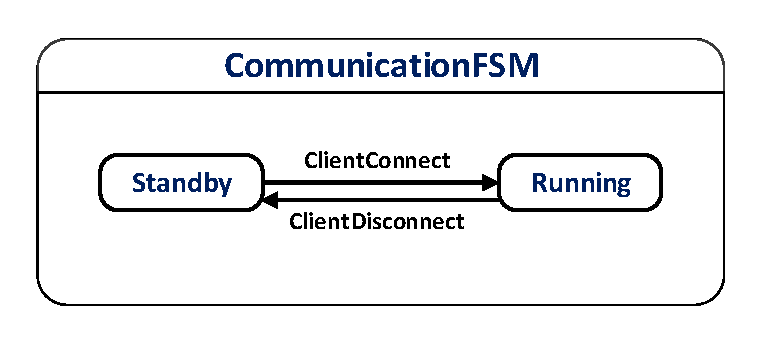
\includegraphics[width=0.7\linewidth]{img/SW_4_CommComp_SC.pdf}
\caption{Zustandsdiagramm der Kommunikations-Komponente}
\end{figure}
Für die Implementierung der Zustandsmaschine wird die objektorientierte Methode nach Samek verwendet (Abschnitt...). An dieser Stelle werden keine Templates verwendet, da die Maschine lediglich zwei Unterstände besitzt. Des weiteren ist nicht zu erwarten, dass sich das Zustandsdiagramm im Entwicklungsprozess verändert.

Der Actionhandler der Zustandsmaschine besitzt eine Instanz der Klasse \textit{CServer}, welche die nötigen Serverfunktionalitäten bereitstellt.
\begin{lstlisting}[caption={Implementierung der Server-Klasse},captionpos=b]
class CServer
{
public:
	void init();
	bool waitForClient();
	bool transmitMessage(CMessage& msg);
	bool receiveMessage(CMessage& msg);
	...
};
\end{lstlisting}
In der \textit{waitForClient()}-Methode wird der aufrufende Thread blockiert bis ein Client eine Verbindung aufbaut. Anschließend können mittels der Methoden \textit{transmitMessage()} und \textit{receiveMessage()} Nachrichten versendet bzw. empfangen werden. Da es sich bei einer TCP/IP-Verbindung um einen Bytestream handelt wird der Typ \textit{CMessage} als Datenpaket in der Übertragung verwendet. Das heißt das lediglich Instanzen von \textit{CMessage} übermittelt werden, wobei die Objekte byteweise versendet und empfangen werden. Im Anschluss werden die einzelnen Bytes wieder zu einer Instanz von \textit{CMessage} zusammengesetzt.

Da das Versenden und Empfangen von Nachrichten parallel erfolgen soll, wird die Kommunikationskomponente um einen zweiten Thread erweitert. Dieser wird in der Klasse \textit{CReceiveTask} implementiert, welche von \textit{IRunnable} erbt. Dieser Thread ist sowohl für das Empfangen von Nachrichten als auch die Annahme von Verbindungsanfragen zuständig.
\begin{lstlisting}[caption={Implementierung des Receive-Tasks},captionpos=b]
void CReceiveTask::run()
{
	while(true)
	{
		if(mServer.waitForClient() == true)
		{
			sProxy.clientConnected();
		}
		
		CMessage receivedMsg;
		while(mServer.receiveMessage(receivedMsg)
		{
			sProxy.routeClientMessage(receivedMsg);
		}
		sProxy.clientDisconnect();
	}
}
\end{lstlisting}
Der Thread ruft zunächst die \textit{waitForClient()}-Methode der \textit{CServer}-Instanz auf, welche den Thread solange blockiert bis eine Verbindung aufgebaut wurde. Daraufhin erzeugt der Task mittels des Proxy ein Ereignis um die Komponente zu benachrichtigen. Im nächsten Schritt ruft der Task die \textit{receiveMessage()}-Methode des Servers in einer Schleife auf. Diese blockiert den Thread bis entweder eine Nachricht eintrifft oder die Verbindung abgebrochen wird. Die Fallunterscheidung erfolgt mit Hilfe des Rückgabewertes von \textit{receiveMessage()}, wobei im Fall einer empfangenen Nachricht diese über den Proxy an die Regelungskomponente weitergeleitet wird. Wird die Verbindung von dem Client abgebrochen verlässt der Task die Empfangsschleife. Anschließend wird der Verbindungsabbruch über den Proxy signalisiert und wieder auf eine erneute Anfrage gewartet.

Der Hauptthread der Komponente wird über deren Eventqueue synchronisiert. Hierbei sind lediglich drei Fälle zu unterscheiden. Die Events \textit{ClientConnect} und \textit{ClientDisconnect} führen jeweils zu einem Zustandswechsel der Zustandsmaschine. Befindet diese sich im Zustand \textit{Running} wird zusätzlich geprüft ob es sich um eine Nachricht handelt, welche über den Server an den Desktop-Client weitergeleitet werden muss.
\newpage
\section{Aufbau der Desktop-Anwendung}
Der letzte Teil der Software-Infrastruktur besteht in einer Anwendung, welche in einer gewöhnlichen Desktopumgebung ausgeführt wird und die Interaktion mit der Zielplattform ermöglicht. In diesem Fall wird als Desktopbetriebssystem Ubuntu 16.04 verwendet. Die Anwendung stellt eine graphische Benutzeroberfläche zur Verfügung, welche einerseits relevante Daten der Versuche visualisiert und andererseits Bedienelemente bietet, um Versuchskonfigurationen vorzunehmen.

Für die Implementierung der Benutzeroberfläche wird die Bibliothek Qt verwendet, welche übliche Bedien- und Grafikelemente zur Verfügung stellt. Der Aufbau der Anwendung ist in zwei Threads unterteilt. Der Erste verwaltet eine Instanz der Klasse \textit{CClient}. Dieses Objekt stellt das Gegenstück zu dem Server dar, der auf dem BeagleBone Black ausgeführt wird. Die Klasse \textit{CClient} bietet ebenfalls die Methoden \textit{receiveMessage()} und \textit{transmitMessage()}, um Nachrichten zu Empfangen bzw. zu Versenden. Zudem kann die Methode \textit{connectToServer()} genutzt werden, um eine Verbindung mit dem BeagleBone Black herzustellen.

Der zweite Thread verwaltet die Benutzeroberfläche. Diese setzt sich aus Plots zur Darstellung der Versuchsdaten und den nötigen Bedienelementen für die Versuchskonfiguration zusammen. Für die Kommunikation zwischen den beiden Threads wird Qts Signal/Slot-Prinzip verwendet. Der Qt-Meta-Compiler ermöglicht es Methoden als Signale bzw. Slots zu deklarieren. In der Anwendung können die Signale eines Objekts mit den Slots eines weiteren Objekts verbunden werden. Anschließend kann ein Objekt seine Signale emittieren, woraufhin der verbundene Slot aufgerufen wird. Als Beispiel sei eine Gruppe von Schalter zur Auswahl des Reglerkonzeptes genannt. Wird einer der Schalter gedrückt, löst dieser ein Signal aus, welches mit einem Slot des Grafik-Threads verbunden ist. In diesem wird die Auswahl ausgewertet und ein entsprechendes Signal ausgelöst. Das Signal des Grafik-Threads ist wiederum an einen Slot des Kommunikations-Threads gekoppelt. In dem Slot wird eine Instanz von \textit{CMessage} mit dem passenden Event angelegt und über den Client an das BeagleBoneBlack gesendet. Umgekehrt wird bei dem Eintreffen von Versuchsdaten ein entsprechendes Signal des Kommunikations-Thread emittiert. In dem zugehörigen Slot des Grafik-Threads werden die Daten verarbeitet und in den Plots angezeigt.

\ifx\FORMAT\undefined
\end{document}
\fi